% Provenance (never printed): see sources/outline_sources.md (Year 2: taphonomy; index fossils;
% facies and fossils as environment markers; reconstructing a palaeoenvironment from a map and a
% section). Taphonomy after Loron (2024); live, dead and fossil assemblages after Tyler and
% Kowalewski (2025); Lagerstaetten after Gaines and others (2024), Mussini and Butterfield
% (2025), Vannier and others (2018), Gerschermann and others (2021) and Rauhut and others
% (2018); zone durations after Al-Suwaidi and others (2022); ichnofacies after Buatois and others
% (2020) and Paz and others (2023); stenohaline groups after McGairy and others (2021) and Saleh
% and others (2022). The Varden column from figdata/shared/region.py; porosities and rates from
% figdata/bachelor-2/palaeoenv.py; exercise and problem values in the Book 4 scratch calculator
% calc/ch20.py. The fossil content given to the Varden units is invented, like the region.
\chapter{Fósseis e paleoambientes}\label{ch:b2:palaeoenvironments}

Numa laje de arenito cinzento há três indícios: a pista que um trilobita arou na lama,
as marcas onduladas que uma corrente deixou e uma toca que um verme escavou e abandonou. Nenhum deles é um
animal inteiro, e no entanto juntos dizem que esta encosta foi um dia o fundo de um mar, raso o
bastante para as ondas o agitarem, salgado o bastante para os trilobitas viverem nele. Os fósseis são os
restos e os vestígios da vida passada, e os geólogos os leem duas vezes: como relógios que datam a rocha
e como testemunhas do lugar onde ela se formou. Este capítulo acompanha um ser vivo desde sua morte
até a gaveta do colecionador, abre os raros depósitos onde até os corpos moles sobrevivem, e depois lê
o ambiente de um mar desaparecido, com números, na cobertura das Varden Hills.
% ledger: usgs:fossil-record-bulk, loron24:taphonomy

\begin{recall}
\textbf{Dos volumes escolares}: fóssil, molde, contramolde e \omterm{def:b2:palaeoenvironments:fossil-kinds}{icnofóssil}; como o soterramento e os minerais
transformam uma concha em pedra; a sucessão dos fósseis ao longo do tempo. \textbf{Do volume do primeiro ano}:
fácies sedimentares e ambientes deposicionais, turbiditos, recifes e oóides; biozonas, fósseis-guia
e datums de primeira ocorrência; compactação, descompactação, a lei de Athy e a espessura sólida
de uma camada; o cimento; a acomodação. \textbf{Dos capítulos anteriores}: as transgressões e regressões,
o nível do mar de longo prazo e os \omterm{def:b2:phanerozoic-earth:oae}{eventos anóxicos oceânicos} (\cref{ch:b2:phanerozoic-earth}). Como as
espécies evoluem, e como os animais e as plantas se classificam, pertence aos livros de biologia.
\end{recall}

\section{Da morte ao fóssil}\label{sec:b2:palaeoenvironments:taphonomy}

A maioria dos seres vivos não deixa nada para trás. Bactérias e necrófagos consomem as partes moles em
dias ou anos, as correntes quebram e espalham as duras, e os ácidos dos solos e das águas intersticiais
dissolvem o que resta. Um fóssil é o que sobrevive a tudo isso, e sobrevive ainda ao soterramento,
ao aquecimento e ao soerguimento da rocha que o contém.

\begin{definition}[Tafonomia; potencial de preservação]\label{def:b2:palaeoenvironments:taphonomy}
A \emph{tafonomia}\index{tafonomia} é o estudo do que acontece aos restos de um organismo
desde sua morte até sua descoberta como fóssil: decomposição, necrofagia, transporte, soterramento e as
mudanças químicas da diagênese. O \emph{potencial de preservação}\index{potencial de preservação}
de um organismo, ou de uma de suas partes, é a probabilidade de que ele passe por essas etapas
e sobreviva na rocha.
\end{definition}
% ledger: loron24:taphonomy

Cada etapa retira algo, acrescenta algo ou muda algo. A decomposição e a necrofagia retiram os
tecidos moles; minerais da água intersticial preenchem os poros de um osso ou substituem a aragonita de uma
concha, acrescentando matéria que o animal nunca teve; o aquecimento altera as moléculas orgânicas que restam.
Loron classifica todas essas mudanças post mortem em três tipos, ganho, perda e alteração, e
as escreve como uma só equação para a variação de qualquer característica mensurável entre um organismo e seu
fóssil. A figura abaixo acompanha as etapas e o que cada uma retira.
% ledger: loron24:taphonomy

\begin{omfigure}
\centering
\begin{tikzpicture}[font=\scriptsize, x=1cm, y=1cm,
  stage/.style={draw=black!60, fill=omSea!12, rounded corners=2pt, align=center,
    text width=2.05cm, minimum height=1.25cm, inner sep=2pt},
  loss/.style={align=center, text width=2.05cm, text=omThm!80!black}]
\node[stage] (a) at (0,0) {\textbf{morte}\\comunidade\\viva};
\node[stage] (b) at (2.75,0) {\textbf{decomposição e}\\\textbf{necrofagia}\\no fundo};
\node[stage] (c) at (5.5,0) {\textbf{transporte}\\as correntes\\selecionam e quebram};
\node[stage] (d) at (8.25,0) {\textbf{soterramento}\\abaixo da\\camada ativa};
\node[stage] (e) at (11,0) {\textbf{diagênese}\\compactação,\\substituição};
\node[stage] (f) at (13.75,0) {\textbf{exumação}\\e\\coleta};
\foreach \u/\v in {a/b, b/c, c/d, d/e, e/f} {\draw[-{Stealth[length=2mm]}, black!70] (\u) -- (\v);}
\node[loss, anchor=north] at (2.75,-0.8) {tecido mole perdido;\\esqueletos se desarticulam};
\node[loss, anchor=north] at (5.5,-0.8) {partes leves levadas,\\conchas quebradas};
\node[loss, anchor=north] at (8.25,-0.8) {soterramento lento: mais\\tempo para as perdas};
\node[loss, anchor=north] at (11,-0.8) {aragonita dissolvida,\\minerais acrescentados};
\node[loss, anchor=north] at (13.75,-0.8) {erodido,\\ou nunca encontrado};
\end{tikzpicture}
\par\smallskip{\small O caminho tafonômico de uma comunidade viva até uma coleção, com o que
cada etapa retira ou muda. O soterramento é o ponto de virada: antes dele os restos estão expostos a
todas as perdas; depois dele, só a diagênese e a erosão agem sobre eles.}
\end{omfigure}
% ledger: loron24:taphonomy

Os volumes escolares chamavam de fóssil qualquer resto ou vestígio de vida passada conservado na rocha. Os dois tipos
comportam-se de modo tão diferente na rocha que merecem nomes próprios.

\begin{definition}[Fóssil corporal; icnofóssil]\label{def:b2:palaeoenvironments:fossil-kinds}
Um \emph{fóssil corporal}\index{fóssil corporal} é uma parte do corpo de um organismo, ou o molde ou o contramolde
dessa parte: uma concha, um osso, um dente, uma folha e, em depósitos raros, um tecido mole. Um
\emph{icnofóssil}\index{icnofóssil} é uma estrutura que um organismo produziu por sua atividade num
sedimento ou numa rocha, ou sobre eles: uma pegada, uma pista, uma toca, uma perfuração, um padrão de alimentação.
\end{definition}

Um \omterm{def:b2:palaeoenvironments:fossil-kinds}{icnofóssil} faz parte do sedimento em que foi escavado: uma corrente que o movesse o destruiria.
Ele registra, portanto, as condições do próprio lugar onde vivia seu produtor, o que uma concha,
facilmente rolada pelo fundo, nem sempre faz. Os \omterm{def:b2:palaeoenvironments:fossil-kinds}{icnofósseis} recebem nomes como os organismos, com um
gênero e uma espécie, mas o nome descreve a estrutura, não o animal: a mesma toca pode ser
escavada por vários tipos de animal, e um animal pode deixar vários tipos de vestígio.

\subsection*{Soterramento contra destruição}

A corrida entre o soterramento e a destruição pode ser posta num modelo simples. Os restos que jazem no
fundo são destruídos a uma taxa constante $k$, a probabilidade por unidade de tempo de serem comidos,
quebrados ou dissolvidos; ficam a salvo quando uma espessura $h$ de sedimento os cobre; e o
sedimento se acumula à taxa $s$.

\begin{proposition}[Soterramento antes da destruição]\label{prop:b2:palaeoenvironments:burial}
Sob essas hipóteses, a probabilidade de que um resto chegue a salvo é
\[
  P = e^{-kh/s}.
\]
Ela depende das três grandezas apenas pela razão entre o tempo até o soterramento, $h/s$, e o
tempo médio de sobrevivência no fundo, $1/k$.
\end{proposition}

\begin{proof}
O resto precisa do tempo $T = h/s$ para ser coberto pela espessura $h$. Com uma taxa constante de
destruição $k$, a probabilidade $p(t)$ de sobreviver até o tempo $t$ obedece a $p' = -kp$, $p(0) =
1$, de modo que $p(t) = e^{-kt}$; em $t = T$ isso dá $e^{-kh/s}$.
\end{proof}

\begin{example}[Uma concha num fundo calmo]\label{ex:b2:palaeoenvironments:shell}
Suponha-se que uma concha sobreviva no fundo 20 anos em média, $k = \qty{0.05}{yr^{-1}}$, e fique
a salvo sob $h = \qty{0.1}{m}$ de lama. Com $s = \qty{1}{mm.yr^{-1}}$ o tempo até o soterramento é de 100
anos e $P = e^{-5} = 0.0067$: menos de uma concha em cem sobrevive. Com
\qty{1}{cm.yr^{-1}}, $P = e^{-0.5} = 0.61$. Uma tempestade que despeja \qty{0.3}{m} de areia num dia
soterra tudo de uma vez, e então $P$ fica perto de um. Os números são supostos, mas a lição
não: os fósseis se concentram onde o sedimento chega depressa ou em camadas súbitas.
\end{example}

O modelo mostra também por que o registro é enviesado. Um verme de corpo mole, cujo tempo médio de sobrevivência no
fundo é de dias e não de décadas, tem um valor de $k$ centenas de vezes maior que uma concha
espessa e, portanto, uma chance exponencialmente menor. O grosso do registro fóssil é feito de animais
com concha e de restos microscópicos. Tyler e Kowalewski testaram quanto uma comunidade perde em
seu caminho para a rocha. Em 51 locais de um fundo marinho costeiro, contaram 135 espécies vivas de
invertebrados, 150 espécies entre as conchas e os esqueletos mortos no fundo, e 112 que
têm também registro fóssil. Os mortos superam os vivos porque as conchas do fundo se acumularam
ao longo de muitos anos, a partir de animais que já não vivem ali. Os detritívoros e os carnívoros, na maioria
de corpo mole, são os que têm menos chance de preservação; ainda assim, os principais grupos ecológicos da comunidade
viva foram todos reencontrados entre os mortos.
% ledger: usgs:fossil-record-bulk, tyler25:live-dead, tyler25:soft-bodied

\section{Janelas de preservação excepcional}\label{sec:b2:palaeoenvironments:lagerstatten}

\begin{definition}[Lagerstätte]\label{def:b2:palaeoenvironments:lagerstatte}
Um \emph{Lagerstätte}\index{Lagerstätte} (plural Lagerstätten) é um depósito sedimentar que
preserva fósseis de qualidade excepcional, em particular os tecidos moles, não biomineralizados, que
a decomposição destrói quase em toda parte; esse depósito é chamado também de Konservat-Lagerstätte.
\end{definition}
% ledger: gaines24:konservat

Os Lagerstätten são raros, mas boa parte do que se sabe dos animais de corpo mole vem deles, e
a primeira grande radiação dos animais, no Cambriano, é mais bem compreendida a partir deles.
% ledger: gaines24:konservat

\subsection*{O Folhelho Burgess}

Em 1909 Charles Walcott esboçou em sua caderneta de campo um pequeno artrópode que encontrara no Folhelho
Burgess, na Colúmbia Britânica. Mais tarde coletou centenas de
espécimes dele, \emph{Waptia}, de um único intervalo de cerca de \qty{2}{m} de espessura, o Phyllopod
Bed; sua descrição moderna apoia-se em mais de 1800 espécimes conservados em dois museus. O Folhelho
Burgess, de cerca de 508 milhões de anos, depositou-se em águas mais profundas, diante de uma íngreme
escarpa submarina. Seus fósseis incluem animais sem concha, preservados como películas achatadas de carbono,
muitas vezes corpos inteiros. Essa preservação está ligada ao soterramento em lamas pobres em oxigênio, que os animais não
bioturbavam e as correntes não retrabalhavam: as perdas da figura acima foram interrompidas de imediato.
% ledger: vannier18:waptia, mussini25:burgess

\begin{omfigure}
\centering
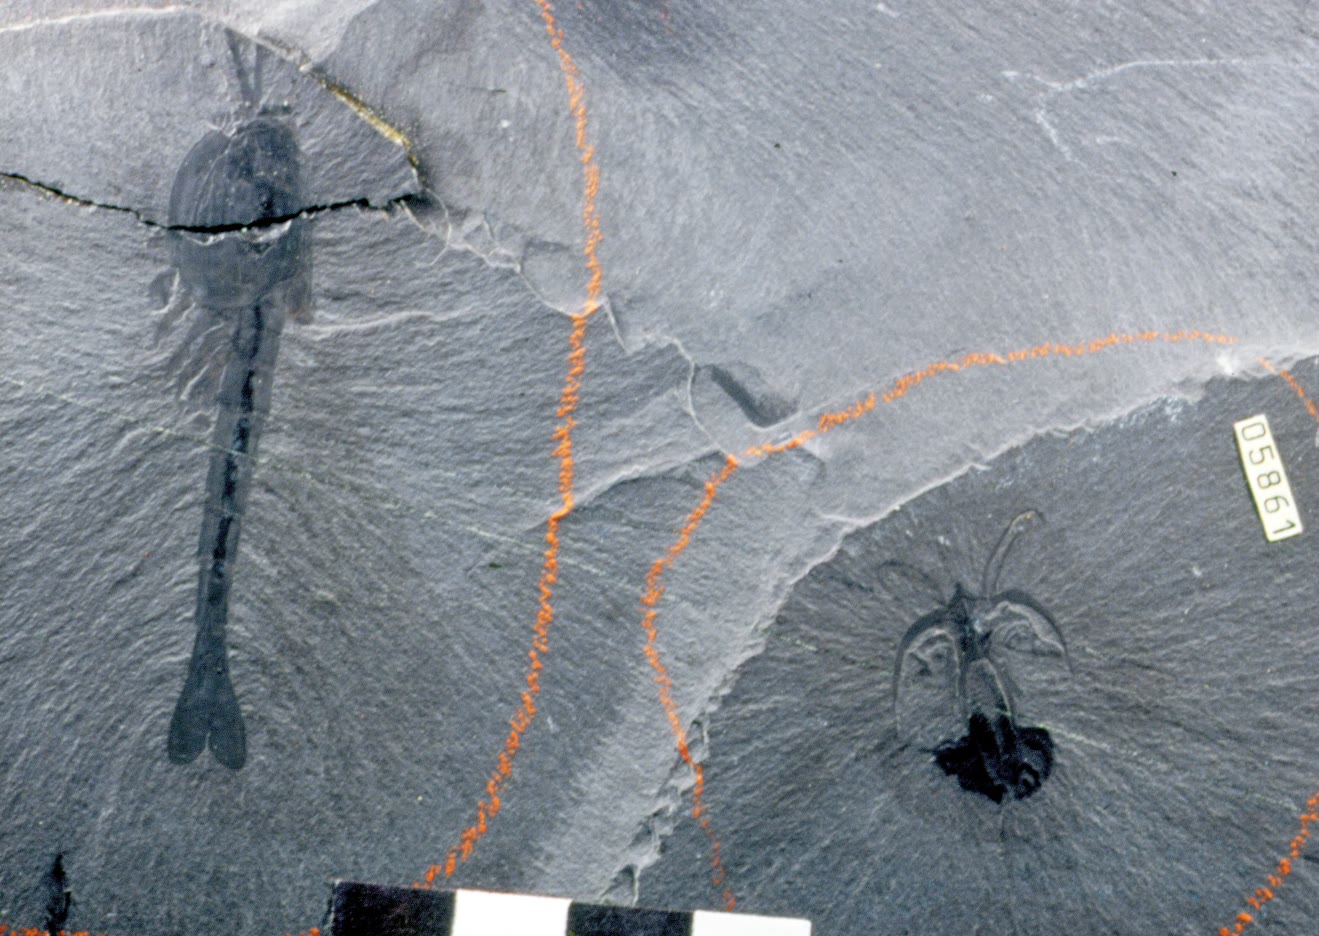
\includegraphics[width=0.72\linewidth]{images/book4/b2-20-burgess-waptia-marrella.jpg}
\par\smallskip{\small Dois artrópodes do Folhelho Burgess, preservados como películas escuras de carbono:
\emph{Waptia} (à esquerda) e \emph{Marrella} (à direita). (Fotografia de James St.~John,
CC~BY~2.0, via Wikimedia Commons.)}
\end{omfigure}
% ledger: mussini25:burgess

\subsection*{Solnhofen}

Os calcários de grão fino de Solnhofen e Eichstätt, na Baviera, depositaram-se em lagunas
no início do Titoniano, a última idade do Jurássico, que começou há \qty{149.2}{Ma}. São
a localidade-tipo de doze espécimes de \emph{Archaeopteryx}, de muitos pterossauros e de peixes
cujos tecidos moles e até padrões de cor sobrevivem. Os fósseis ali são raros, mas sua
preservação é notável. Foram propostas várias condições, talvez agindo em conjunto:
águas de fundo cerca de três vezes mais salgadas que a água do mar ou muito alcalinas, que retardam a
decomposição bacteriana; esteiras de bactérias que selaram as carcaças; água de fundo sem oxigênio, que mantinha
os necrófagos afastados; e tempestades que revolviam a lama calcária e soterravam as carcaças depressa. Cada
uma delas alonga o tempo de sobrevivência $1/k$ ou encurta o tempo até o soterramento $h/s$.
% ledger: gerschermann21:solnhofen, rauhut18:archaeopteryx, ics4:jurassic-stages

\begin{omfigure}
\centering
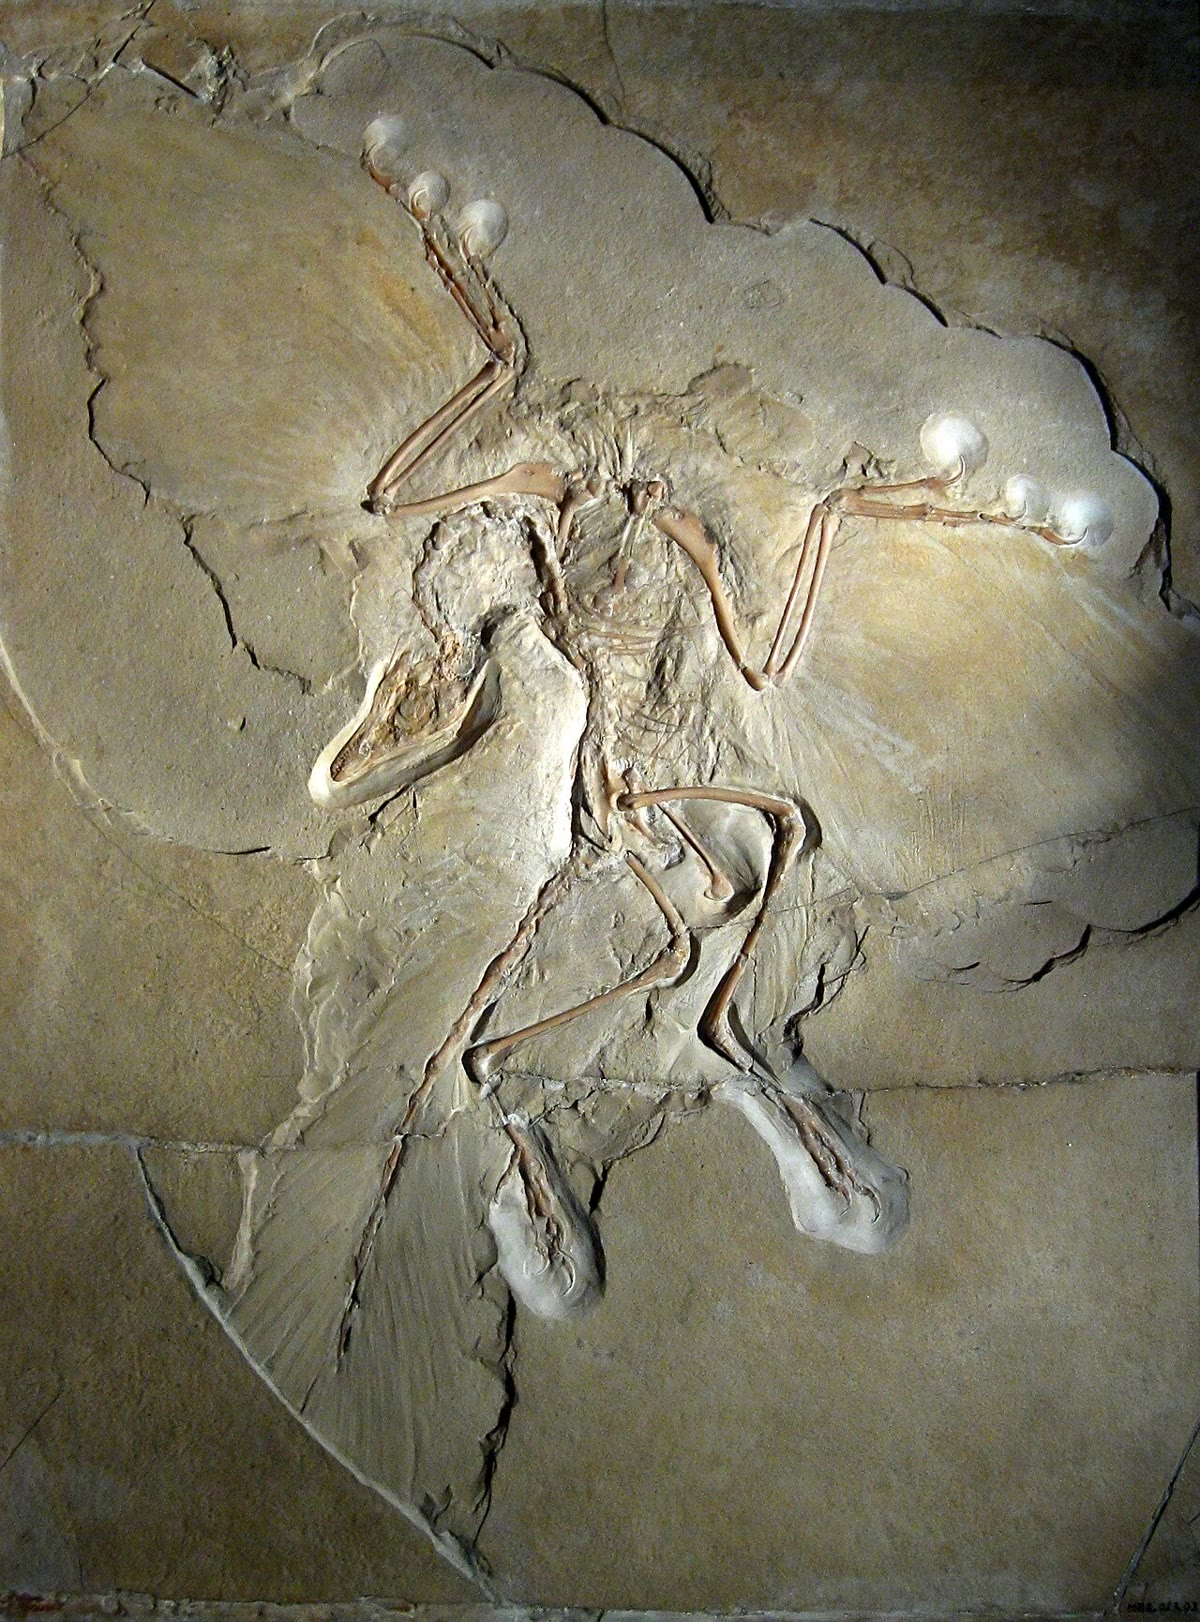
\includegraphics[width=0.5\linewidth]{images/book4/b2-20-archaeopteryx-berlin.jpg}
\par\smallskip{\small O espécime de Berlim do \emph{Archaeopteryx}, dos calcários de Solnhofen:
os ossos e as impressões das penas das asas e da cauda. (H.~Raab, CC~BY-SA~3.0,
via Wikimedia Commons.)}
\end{omfigure}
% ledger: rauhut18:archaeopteryx, gerschermann21:solnhofen

\subsection*{Os fósseis como relógios}

O volume do primeiro ano construiu a biozona, um corpo de estratos definido por seus fósseis, e o fóssil-guia
que a reconhece. Que precisão têm esses relógios? Uma zona de amonites do Jurássico pode durar
cerca de um milhão de anos: a primeira zona do Toarciano, datada com idades urânio--chumbo de camadas de cinza na
Argentina, vai de 183.73 a \qty{182.77}{Ma}. As zonas dividem-se em horizontes, e no Jurássico
Superior um horizonte de amonites dura em média \qty{165}{kyr}. Todos os esqueletos de
\emph{Archaeopteryx} vêm de uma única zona que contém cinco horizontes, de modo que a ave é conhecida ao longo de
uns 0.7 a 1 milhão de anos. Os fósseis, porém, dão apenas uma ordem; as idades em anos vêm
de camadas de cinza datadas por urânio e chumbo, e de ciclos sedimentares. As mesmas camadas de cinza põem a base do Toarciano em $183.73$, com uma incerteza de
$+0.35$ e \qty{-0.50}{Myr}, onde a carta internacional dá \qty{184.2}{Ma}.
% ledger: alsuwaidi22:toarcian, rauhut18:archaeopteryx, ics4:jurassic-stages

\section{Os fósseis como testemunhas do ambiente}\label{sec:b2:palaeoenvironments:environment}

Para ler um ambiente num fóssil, um geólogo supõe que o organismo vivia onde vivem seus parentes
atuais, e que os processos que agem sobre o sedimento hoje agiam da mesma maneira então.

\begin{definition}[Atualismo]\label{def:b2:palaeoenvironments:actualism}
O \emph{atualismo}\index{atualismo} é o método de interpretar os registros geológicos passados pelos
processos, e pelas relações entre os organismos e seu ambiente, que se podem observar hoje.
\end{definition}

Em 1830 Charles Lyell deu ao primeiro volume de seus \emph{Principles of Geology} o subtítulo ``uma
tentativa de explicar as antigas mudanças da superfície da Terra por referência a causas agora em
ação''. O método tem limites. Muitos grupos estão extintos, e seu modo de vida tem de ser
inferido de sua forma e do sedimento à sua volta; e um ambiente do passado pode
não ter equivalente exato hoje.
% ledger: lyell1830:title

\begin{definition}[Paleoambiente]\label{def:b2:palaeoenvironments:palaeoenvironment}
Um \emph{paleoambiente}\index{paleoambiente} é o conjunto das condições físicas, químicas e
biológicas que prevaleciam onde e quando uma rocha se formou: o contexto, a profundidade e a
energia da água, sua salinidade, temperatura e oxigênio, a natureza do fundo, e a vida
sobre ele.
\end{definition}

\subsection*{Onde vivia o fóssil?}

A primeira pergunta é se os fósseis viviam onde jazem.

\begin{definition}[Assembleias de vida e de morte; fósseis autóctones e alóctones]\label{def:b2:palaeoenvironments:assemblages}
Uma \emph{assembleia de vida}\index{assembleia de vida} é um grupo de fósseis de organismos que viviam
juntos, preservados onde e como viviam; uma \emph{assembleia de morte}\index{assembleia de morte} é
um grupo de restos reunidos depois da morte, que pode misturar organismos de lugares diferentes
e de épocas diferentes. Um fóssil é \emph{autóctone}\index{fóssil autóctone} se está
preservado onde o organismo vivia, e \emph{alóctone}\index{fóssil alóctone} se foi
transportado de outro lugar antes do soterramento.
\end{definition}

Os indícios são os do transporte. Conchas ainda fechadas, um coral ou um bivalve escavador em sua
posição de crescimento, espinhos delicados intactos, todas as idades de uma população presentes: os fósseis são
provavelmente \omterm{def:b2:palaeoenvironments:assemblages}{autóctones}. Valvas isoladas selecionadas por tamanho, fragmentos gastos e quebrados, conchas
concentradas na base de uma camada gradada: foram transportados. Uma \omterm{def:b2:palaeoenvironments:assemblages}{assembleia de morte} de conchas, como
a do fundo costeiro acima, ainda contém a maior parte da comunidade, mas reúne muitos anos
dela numa só camada: seus fósseis são médias no tempo.
% ledger: tyler25:live-dead

\subsection*{Salinidade e oxigênio}

Alguns animais só toleram a salinidade do mar aberto: são chamados estenoalinos. Os equinodermos,
os cefalópodes, os corais e, no Paleozoico, os trilobitas são grupos estenoalinos típicos; sua
presença indica água do mar normal, e sua ausência numa fauna rica pode indicar o contrário.
Os depósitos de um estuário siluriano no Vietnã contêm restos vegetais, ossos de peixe, bivalves, gastrópodes
e ostracodes, mas nenhum desses grupos. Os equinodermos também faltam na biota de Chengjiang,
um \omterm{def:b2:palaeoenvironments:lagerstatte}{Lagerstätte} de cerca de 518 milhões de anos, embora ocorram em Lagerstätten de mar aberto do
Cambriano: os animais de Chengjiang viviam ao largo de um delta, onde a água doce fazia a salinidade flutuar.
% ledger: mcgairy21:stenohaline, saleh22:echinoderms, saleh22:age

O oxigênio deixa sua marca pelos escavadores. Onde a água de fundo tem oxigênio, os animais misturam o
sedimento e destroem sua laminação fina; onde não tem, as lâminas sobrevivem, as tocas estão
ausentes e forma-se pirita, como nos folhelhos negros dos \omterm{def:b2:phanerozoic-earth:oae}{eventos anóxicos oceânicos} do
\cref{ch:b2:phanerozoic-earth}. A mesma falta de escavadores protegeu as carcaças do Folhelho
Burgess.
% ledger: mussini25:burgess

\subsection*{Icnofácies}

Os \omterm{def:b2:palaeoenvironments:fossil-kinds}{icnofósseis} são as melhores testemunhas do fundo, porque não foram movidos. Seus produtores
respondem à energia da água, à firmeza do fundo, ao alimento e ao oxigênio, e as
mesmas associações de vestígios repetem-se ao longo do Fanerozoico.

\begin{definition}[Icnofácies]\label{def:b2:palaeoenvironments:ichnofacies}
Uma \emph{icnofácies}\index{icnofácies} é uma associação recorrente de \omterm{def:b2:palaeoenvironments:fossil-kinds}{icnofósseis} que
reflete um conjunto de condições ambientais; recebe o nome de um vestígio característico.
\end{definition}

Ao longo de um perfil marinho, da costa à bacia profunda, quatro \omterm{def:b2:palaeoenvironments:ichnofacies}{icnofácies} marinhas sucedem-se
(figura abaixo). A \omterm{def:b2:palaeoenvironments:ichnofacies}{icnofácies} \emph{Skolithos}, dominada por tocas de habitação verticais, cilíndricas ou
em U, de suspensívoros, com poucos vestígios horizontais, é típica do
estirâncio e da antepraia. A \omterm{def:b2:palaeoenvironments:ichnofacies}{icnofácies} \emph{Cruziana}, dominada pelas tocas de
detritívoros, com os vestígios de pastadores, carnívoros e suspensívoros, é típica da zona
costa afora: o fundo entre o nível de base das ondas de tempo bom, a profundidade acima da qual as ondas comuns agitam
o sedimento, e o nível de base das ondas de tempestade, atingido apenas pelas ondas de tempestade. A \omterm{def:b2:palaeoenvironments:ichnofacies}{icnofácies}
\emph{Zoophycos}, cujo nome vem de uma toca que retrabalha o sedimento em lâminas helicoidais em torno de um eixo
central, é típica da plataforma abaixo do nível de base das ondas de tempestade e do talude. A \omterm{def:b2:palaeoenvironments:ichnofacies}{icnofácies}
\emph{Nereites}, com suas tocas regulares meandrantes, espirais e em rede, lidas como as armadilhas e os
jardins de animais que encontravam pouco alimento, é típica do mar profundo além da quebra da plataforma. Nas
baías salobras e nos estuários, a regra é uma \omterm{def:b2:palaeoenvironments:ichnofacies}{icnofácies} Cruziana com poucas espécies.
% ledger: buatois20:ichnofacies, miguez21:ichnofacies, zhang15:zoophycos, buatois25:graphoglyptids, paz23:nereites

\begin{omfigure}
\centering
\begin{tikzpicture}[font=\scriptsize, x=1cm, y=1cm]
% sea and floor (schematic, not to scale)
\fill[omSea!20] (0.6,0) -- (14,0) -- (14,-3.6) -- (11.2,-3.6) -- (9.6,-1.9) -- (6.2,-1.5)
  -- (3.2,-0.9) -- (1.2,-0.15) -- cycle;
\fill[omLithSand!45] (0,0.25) -- (0.6,0) -- (1.2,-0.15) -- (3.2,-0.9) -- (6.2,-1.5)
  -- (9.6,-1.9) -- (11.2,-3.6) -- (14,-3.6) -- (14,-4.3) -- (0,-4.3) -- cycle;
\draw[black!70, line width=0.6pt] (0,0.25) -- (0.6,0) -- (1.2,-0.15) -- (3.2,-0.9) -- (6.2,-1.5)
  -- (9.6,-1.9) -- (11.2,-3.6) -- (14,-3.6);
\draw[omSea!80!black, line width=0.6pt] (0.6,0) -- (14,0);
\node[anchor=south east, omSea!80!black] at (14,0) {nível do mar};
% wave bases
\draw[dashed, black!60] (2.133,-0.5) -- (14,-0.5) node[anchor=south east, black!70] {nível de base das ondas de tempo bom};
\draw[dashed, black!60] (4.7,-1.2) -- (14,-1.2) node[anchor=south east, black!70] {nível de base das ondas de tempestade};
% zone labels
\node[align=center] at (1.9,0.55) {estirâncio,\\antepraia};
\node[align=center] at (4.6,0.55) {costa afora};
\node[align=center] at (8.0,0.55) {plataforma};
\node[align=center] at (10.5,0.55) {talude};
\node[align=center] at (12.7,0.55) {bacia};
% Skolithos: vertical tubes
\foreach \x in {1.75,1.95,2.15,2.35} {\draw[black!80, line width=0.7pt] (\x,{-0.15-0.375*(\x-1.2)}) -- ++(0,-0.55);}
\node[align=center] at (2.1,-2.15) {\textbf{\emph{Skolithos}}\\tubos verticais};
% Cruziana: horizontal bilobed trails
\foreach \x in {4.0,4.8} {\draw[black!80, line width=0.6pt] (\x,-1.45) .. controls ++(0.2,0.08) .. ++(0.5,0);
  \draw[black!80, line width=0.6pt] (\x,-1.53) .. controls ++(0.2,-0.08) .. ++(0.5,0);}
\node[align=center] at (4.7,-2.35) {\textbf{\emph{Cruziana}}\\tocas de alimentação,\\pistas de pastagem};
% Zoophycos: spreite arcs
\foreach \r in {0.12,0.22,0.32} {\draw[black!80, line width=0.5pt] (8.0,-2.25) ++(-\r,0) arc (180:360:\r cm and 0.5*\r cm);}
\draw[black!80, line width=0.6pt] (8.0,-2.25) -- (8.0,-1.8);
\node[align=center] at (8.0,-3.05) {\textbf{\emph{Zoophycos}}\\lâminas\\helicoidais};
% Nereites: meander
\draw[black!80, line width=0.6pt, domain=0:2.2, samples=80, smooth] plot (12.0+\x*0.5,{-3.9+0.12*sin(\x*720)});
\node[align=center, anchor=north] at (12.5,-4.35) {\textbf{\emph{Nereites}}\\meandros, redes};
\end{tikzpicture}
\par\smallskip{\small As quatro \omterm{def:b2:palaeoenvironments:ichnofacies}{icnofácies} marinhas do modelo de Seilacher ao longo de um perfil da
costa à bacia profunda, com o esboço de um vestígio característico de cada uma; as profundidades estão fora de
escala. Os vestígios respondem à energia, ao alimento e ao oxigênio mais do que à profundidade em si.}
\end{omfigure}
% ledger: buatois20:ichnofacies, miguez21:ichnofacies, zhang15:zoophycos, buatois25:graphoglyptids, paz23:nereites

A profundidade não age diretamente. Num canal de mar profundo, onde as correntes de turbidez são fortes, tocas
verticais da \omterm{def:b2:palaeoenvironments:ichnofacies}{icnofácies} Skolithos aparecem muito abaixo de qualquer nível de base das ondas; e perto de um delta, onde a água
doce e a lama afluem, os vestígios de costa afora são mais pobres que em outros lugares. Os produtores também se deslocaram
ao longo do tempo: a toca \emph{Zoophycos} vivia na plataforma no Paleozoico, na plataforma inferior
e no talude no Mesozoico, e no mar profundo no Cenozoico. Uma \omterm{def:b2:palaeoenvironments:ichnofacies}{icnofácies} registra as
condições no fundo, das quais a profundidade é apenas inferida, e a inferência deve levar em conta
a idade da rocha.
% ledger: buatois20:ichnofacies, zhang15:zoophycos

\begin{inthefield}[Contar fósseis camada por camada]
Um paleontólogo que reconstrói um ambiente a partir de uma seção registra cada camada com sua
litologia, espessura e estruturas sedimentares, e depois seus fósseis: que grupos, quantos,
se as conchas estão inteiras ou quebradas, fechadas ou abertas, selecionadas ou não, e em que posição jazem.
Os \omterm{def:b2:palaeoenvironments:fossil-kinds}{icnofósseis} são registrados onde são vistos, nas superfícies de acamamento e nas faces verticais,
com a profundidade que as tocas atingem. Como uma concha pode ser movida e uma toca não, as
duas listas são mantidas à parte; o ambiente é lido primeiro nos vestígios, e os \omterm{def:b2:palaeoenvironments:fossil-kinds}{fósseis corporais}
são depois examinados em busca de sinais de transporte.
\end{inthefield}

\begin{omfigure}
\centering
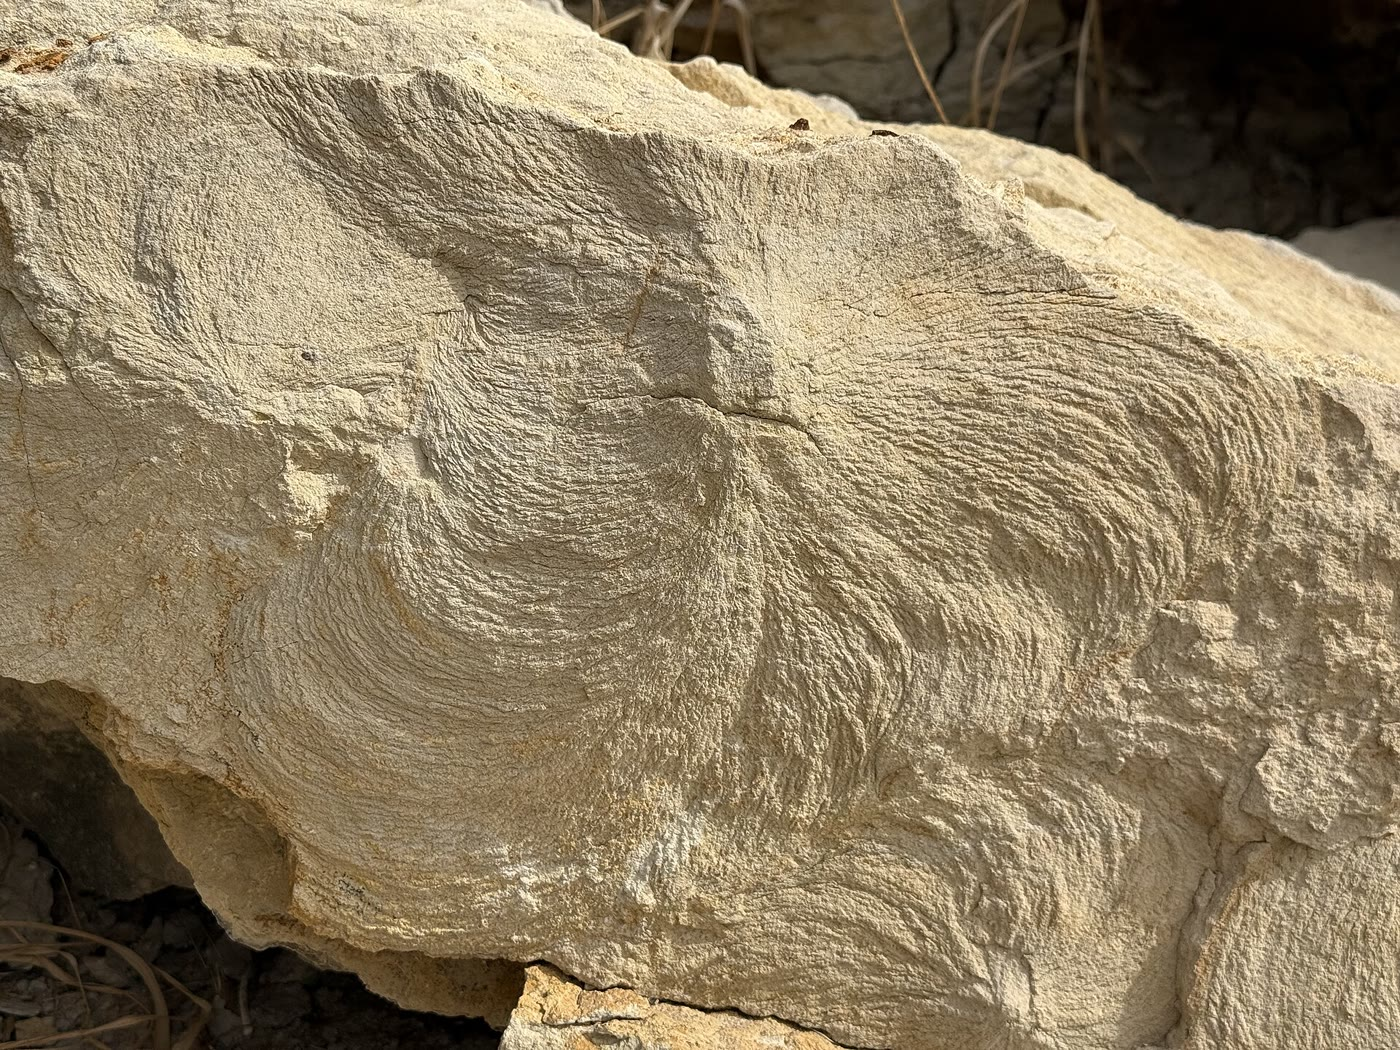
\includegraphics[width=0.5\linewidth]{images/book4/b2-20-zoophycos.jpg}
\par\smallskip{\small \emph{Zoophycos} num bloco em Sagres, Portugal: os arcos são as lamelas
de uma lâmina helicoidal de sedimento retrabalhado. (Amada44, CC~BY~4.0, via Wikimedia Commons.)}
\end{omfigure}
% ledger: zhang15:zoophycos

\section{Ler um mar desaparecido}\label{sec:b2:palaeoenvironments:varden}

Os ambientes ficam lado a lado: uma praia, um fundo costa afora, uma plataforma mais profunda. Quando o mar sobe ou
o fundo afunda, cada ambiente avança em direção ao continente sobre seu vizinho, e seus depósitos passam a ficar
sobre os do vizinho. Uma sucessão vertical de fácies, sem interrupção, repete assim
a ordem dos ambientes que ficavam lado a lado; o volume do terceiro ano faz dessa regra,
a lei de Walther, seu ponto de partida. Um perfil lido de baixo para cima é um filme da costa deslocando-se
sobre um mesmo lugar.

A cobertura das Varden Hills, a região inventada da série, dá um exemplo completo. Suas
espessuras são as do modelo da região; os fósseis da figura abaixo foram inventados para ela,
mas cada um foi escolhido entre os que rochas reais desse tipo podem conter. Ao calcário atribui-se o
Toarciano, de 184.2 a \qty{174.7}{Ma}, e ao folhelho do Aaleniano ao Caloviano, de
\qty{174.7}{Ma} a \qty{161.5}{Ma}.
% ledger: data:b4-palaeoenv, ics4:jurassic-stages

\begin{omfigure}
\centering
% figdata/bachelor-2/palaeoenv.py part log (thicknesses from figdata/shared/region.py)
\begin{tikzpicture}[x=1cm, y=0.0165cm, font=\scriptsize]
% scale
\draw[black!70] (-0.35,0) -- (-0.35,460);
\foreach \z in {0,100,...,400} {\draw[black!70] (-0.45,\z) -- (-0.35,\z) node[left=3pt] {\z};}
\node[rotate=90, anchor=south] at (-1.15,230) {altura acima da base da cobertura (m)};
% units
\fill[lith sandstone] (0,0) rectangle (2.2,120);
\fill[lith limestone] (0,120) rectangle (2.0,180);
\fill[lith limestone] (0,180) rectangle (1.6,300);
\fill[lith shale] (0,300) rectangle (1.1,400);
\fill[om lith={icsCretaceous!35}{om limestone}] (0,400) -- (1.4,400) -- (1.4,452)
  .. controls (1.0,466) and (0.6,446) .. (0.3,458) -- (0,455) -- cycle;
\draw[black!70] (0,0) rectangle (2.2,120);
\draw[black!70] (0,120) rectangle (2.0,180);
\draw[black!70] (0,180) rectangle (1.6,300);
\draw[black!70] (0,300) rectangle (1.1,400);
\draw[black!70] (0,400) -- (1.4,400) -- (1.4,452) .. controls (1.0,466) and (0.6,446) ..
  (0.3,458) -- (0,455) -- cycle;
\node[anchor=west, font=\tiny] at (1.45,460) {topo erodido};
% unit names
\node[anchor=west, align=left] at (2.6,60) {\textbf{arenito}, \qty{120}{m}\\Triássico};
\node[anchor=west, align=left] at (2.6,150) {\textbf{calcário oolítico}, \qty{60}{m}\\Toarciano};
\node[anchor=west, align=left] at (2.6,240) {\textbf{calcário fino}, \qty{120}{m}\\Toarciano};
\node[anchor=west, align=left] at (2.6,350) {\textbf{folhelho}, \qty{100}{m}\\Aaleniano--Caloviano};
\node[anchor=west, align=left] at (2.6,424) {\textbf{giz}\\Cretáceo};
% content
\node[anchor=west, align=left, text width=6.9cm] at (6.3,60) {preenchimentos de canal com estratificação cruzada sobre bases
  erosivas; marcas de raízes; fragmentos vegetais; nenhum fóssil marinho};
\node[anchor=west, align=left, text width=6.9cm] at (6.3,150) {oóides com estratificação cruzada; tubos verticais
  e tocas em U; fragmentos de concha gastos};
\node[anchor=west, align=left, text width=6.9cm] at (6.3,240) {ossículos de crinoides, braquiópodes,
  belemnites, amonites; pistas de rastejamento e tocas de alimentação; camadas de conchas quebradas com bases
  abruptas};
\node[anchor=west, align=left, text width=6.9cm] at (6.3,350) {cinza-escuro, laminado em partes;
  pirita; amonites e bivalves de concha fina; tocas com spreite helicoidal nas camadas mais claras};
\node[anchor=west, align=left, text width=6.9cm] at (6.3,424) {cocólitos; equinoides, esponjas;
  nódulos de sílex; bioturbado em toda a espessura};
\foreach \z in {120,180,300,400} {\draw[black!25] (2.25,\z) -- (13.2,\z);}
\node[font=\scriptsize\bfseries, anchor=south west] at (2.6,462) {unidade e idade};
\node[font=\scriptsize\bfseries, anchor=south west] at (6.3,462) {o que as camadas contêm};
\end{tikzpicture}
\par\smallskip{\small A cobertura das Varden Hills como perfil, com o conteúdo de suas unidades. As
espessuras são as do modelo da região, exceto a do giz, cujo topo erodido aparece cortado aqui
(\qty{766}{m} de espessura no sinclinal do \cref{ex:b2:palaeoenvironments:shale}); a largura da coluna cresce com o tamanho do grão;
os fósseis e suas idades foram inventados para a região.}
\end{omfigure}
% ledger: data:b4-palaeoenv, ics4:jurassic-stages

\begin{example}[A base da cobertura de Varden]\label{ex:b2:palaeoenvironments:base}
O arenito contém preenchimentos de canal sobre bases erosivas, raízes e fragmentos vegetais, e nenhum fóssil
marinho: foi depositado por rios em terra. O calcário oolítico acima tem oóides com estratificação cruzada,
que crescem rolando em água agitada, tubos verticais e tocas em U da \omterm{def:b2:palaeoenvironments:ichnofacies}{icnofácies}
Skolithos, e fragmentos de concha gastos, todos \omterm{def:b2:palaeoenvironments:assemblages}{alóctones}: um baixio da antepraia,
varrido pelas ondas. Entre os dois o mar chegou: o contato registra uma \omterm{def:b2:phanerozoic-earth:transgression}{transgressão marinha}. Na
ordem da lei de Walther, à planície fluvial seguiu-se a costa, e depois o baixio.
\end{example}
% ledger: buatois20:ichnofacies

\subsection*{Com que rapidez o fundo marinho se encheu?}

Uma biozona dá uma duração, um perfil dá uma espessura, e sua razão é uma taxa. Mas a
espessura diminuiu desde que o sedimento se depositou: a água dos poros foi expulsa,
e só os grãos se conservam.

\begin{proposition}[Taxa de acumulação de uma camada compactada]\label{prop:b2:palaeoenvironments:rate}
Uma camada de espessura atual $h$ e porosidade média $\varphi$, depositada durante o tempo $\Delta t$
com a porosidade $\varphi_0$, acumulou-se à taxa
\[
  r = \frac{h\,(1 - \varphi)}{(1 - \varphi_0)\,\Delta t}
\]
de sedimento fresco, e à taxa $h(1-\varphi)/\Delta t$ de grãos, que não depende de
$\varphi_0$.
\end{proposition}

\begin{proof}
Por unidade de área, a camada contém o volume de grãos $h(1 - \varphi)$, a espessura sólida do
volume do primeiro ano. A compactação expulsa água mas não acrescenta nem retira grãos, de modo que o sedimento
fresco, de porosidade $\varphi_0$, tinha a espessura $h_0$ com $h_0(1 - \varphi_0) = h(1 -
\varphi)$. Dividindo $h_0$ e a espessura sólida por $\Delta t$ obtêm-se as duas taxas.
\end{proof}

Quando a porosidade não foi medida, a lei de Athy a dá a partir da profundidade. A figura abaixo mostra
a lei para quatro litologias, e o fator $(1 - \varphi(z))/(1 - \varphi_0)$ pelo qual uma camada
fina hoje à profundidade $z$ deve ser esticada para dar sua espessura na superfície. O giz e o folhelho
começam com muita água e a perdem depressa: uma camada fina de folhelho a \qty{1000}{m} era 1.68 vezes
mais espessa quando se depositou, uma camada de giz 2.19 vezes.
% ledger: pybacktrack:compaction, pybacktrack4:limestone, data:b4-palaeoenv

\begin{omfigure}
\centering
% figdata/bachelor-2/palaeoenv.py parts poro and ratio
\begin{tikzpicture}
\begin{groupplot}[group style={group size=2 by 1, horizontal sep=1.6cm},
  width=0.46\linewidth, height=6.2cm, y dir=reverse, ymin=0, ymax=3000,
  tick label style={font=\scriptsize}, label style={font=\small}, xtick pos=bottom,
  ytick pos=left, scaled y ticks=false, yticklabel style={/pgf/number format/1000 sep={\,}}]
\nextgroupplot[xmin=0, xmax=0.75, xlabel={porosidade $\varphi$}, ylabel={profundidade $z$ (\unit{m})},
  legend style={at={(0.5,1.04)}, anchor=south, draw=none, font=\scriptsize, legend columns=2}]
\addplot[omThm, line width=1pt] table[x=shale, y=z_m] {figdata/out/bachelor-2-palaeoenv-poro.dat};
\addlegendentry{folhelho}
\addplot[omSea!80!black, line width=1pt, dashed] table[x=sandstone, y=z_m] {figdata/out/bachelor-2-palaeoenv-poro.dat};
\addlegendentry{arenito}
\addplot[black, line width=1pt, dotted] table[x=chalk, y=z_m] {figdata/out/bachelor-2-palaeoenv-poro.dat};
\addlegendentry{giz}
\addplot[green!45!black, line width=1pt, dash dot] table[x=limestone, y=z_m] {figdata/out/bachelor-2-palaeoenv-poro.dat};
\addlegendentry{calcário}
\nextgroupplot[xmin=1, xmax=3.2, xlabel={fator de restauração $(1-\varphi)/(1-\varphi_0)$}]
\addplot[omThm, line width=1pt] table[x=shale, y=z_m] {figdata/out/bachelor-2-palaeoenv-ratio.dat};
\addplot[omSea!80!black, line width=1pt, dashed] table[x=sandstone, y=z_m] {figdata/out/bachelor-2-palaeoenv-ratio.dat};
\addplot[black, line width=1pt, dotted] table[x=chalk, y=z_m] {figdata/out/bachelor-2-palaeoenv-ratio.dat};
\addplot[green!45!black, line width=1pt, dash dot] table[x=limestone, y=z_m] {figdata/out/bachelor-2-palaeoenv-ratio.dat};
\end{groupplot}
\end{tikzpicture}
\par\smallskip{\small Esquerda: porosidade em função da profundidade pela lei de Athy, com as constantes de Sclater
e Christie (1980) para o folhelho, o arenito e o giz e de Turer e Maynard (2003) para o calcário,
tal como tabuladas no pyBacktrack. Direita: o fator pelo qual uma camada fina à profundidade $z$ é
restaurada à sua espessura na superfície.}
\end{omfigure}
% ledger: pybacktrack:compaction, pybacktrack4:limestone, data:b4-palaeoenv

\begin{example}[O folhelho de Varden]\label{ex:b2:palaeoenvironments:shale}
No sinclinal das Varden Hills o giz tem \qty{766}{m} de espessura, de modo que o folhelho fica entre
766 e \qty{866}{m}. Com as constantes do folhelho, $\varphi_0 = 0.63$ e $\lambda =
\qty{1960}{m}$, a espessura sólida do volume do primeiro ano é $100 - 0.63 \times 1960 \times
(e^{-766/1960} - e^{-866/1960}) = \qty{58.4}{m}$, uma porosidade média de 0.416. Trazida de volta à
superfície com os mesmos grãos, a camada tem \qty{148.6}{m} de espessura. Ao longo dos \qty{13.2}{Myr} da
base do Aaleniano ao topo do Caloviano, o folhelho acumulou-se a $100/13.2 =
\qty{7.6}{m}$ por milhão de anos tal como está hoje, a $148.6/13.2 = \qty{11.3}{m}$ por milhão de
anos de lama fresca, e a \qty{4.4}{m} por milhão de anos de grãos. A espessura atual
subestima a taxa em um terço.
\end{example}
% ledger: data:b4-palaeoenv, pybacktrack:compaction, ics4:jurassic-stages

O folhelho pode ter estado ainda mais fundo, sob giz depois erodido; a correção é então um
mínimo. O problema de fim de semana aplica a proposição ao calcário, onde a porosidade foi
medida.

\section*{Exercícios}\label{sec:b2:palaeoenvironments:exercises}

Dados para os exercícios, salvo indicação em contrário: lei de Athy $\varphi = \varphi_0 e^{-z/\lambda}$
com $\varphi_0 = 0.63$, $\lambda = \qty{1960}{m}$ (folhelho), $0.49$, \qty{3704}{m} (arenito),
$0.70$, \qty{1408}{m} (giz), $0.51$, \qty{4545}{m} (calcário); calcita \qty{2710}{kg.m^{-3}},
água intersticial \qty{1000}{kg.m^{-3}}; as idades da carta internacional: Toarciano de 184.2 a
\qty{174.7}{Ma}.
% ledger: pybacktrack:compaction, pybacktrack4:limestone, ics4:jurassic-stages

\begin{exercise}[$\star$]\label{exo:b2:palaeoenvironments:1}
Em 51 locais de um fundo costeiro, 135 espécies de invertebrados foram encontradas vivas, 150 entre as conchas
e os esqueletos mortos no fundo, e 112 que têm também registro fóssil. (a) Exprima o terceiro
número como fração de cada um dos dois primeiros. (b) Como os mortos podem superar os vivos? (c)
Que grupos alimentares você esperaria encontrar sub-representados entre os mortos, e por quê?
\end{exercise}
% ledger: tyler25:live-dead, tyler25:soft-bodied

\begin{exercise}[$\star$]\label{exo:b2:palaeoenvironments:2}
Um horizonte de amonites do Jurássico Superior dura em média \qty{165}{kyr}. (a) Quanto duram cinco horizontes?
Compare com os 0.7 a 1 milhão de anos dados para o \emph{Archaeopteryx}. (b) A primeira
zona do Toarciano vai de 183.73 a \qty{182.77}{Ma}: quantos horizontes de duração média ela conteria?
(c) Por que os horizontes, e não as zonas, importam para acompanhar a evolução de uma linhagem?
\end{exercise}
% ledger: rauhut18:archaeopteryx, alsuwaidi22:toarcian

\begin{exercise}[$\star$]\label{exo:b2:palaeoenvironments:3}
Nomeie a \omterm{def:b2:palaeoenvironments:ichnofacies}{icnofácies} e o contexto de cada conjunto. (a) Pistas de pastagem meandrantes e redes regulares de
tocas nas bases de turbiditos finos. (b) Tubos verticais muito próximos em areia limpa
com estratificação cruzada. (c) Tocas horizontais abundantes de detritívoros e pistas de pastagem em camadas
siltosas entre areias de tempestade. (d) Tocas com spreite helicoidal numa lama fina e escura sem marcas
onduladas de ondas, em rochas mesozoicas.
\end{exercise}
% ledger: buatois20:ichnofacies, paz23:nereites

\begin{exercise}[$\star$]\label{exo:b2:palaeoenvironments:4}
A camada A contém crinoides, braquiópodes, corais e trilobitas; a camada B, da mesma idade, contém restos
vegetais, ossos de peixe, alguns bivalves e gastrópodes, e muitos indivíduos de apenas duas espécies de
ostracodes. (a) O que cada uma diz sobre a salinidade de sua água? (b) À camada B faltam os grupos da
camada A: por que essa ausência é um argumento, enquanto a ausência de um fóssil numa camada não é?
(c) Que outras observações testariam a interpretação da camada B?
\end{exercise}
% ledger: mcgairy21:stenohaline, saleh22:echinoderms

\begin{exercise}[$\star\star$]\label{exo:b2:palaeoenvironments:5}
Use a \cref{prop:b2:palaeoenvironments:burial} com a concha do
\cref{ex:b2:palaeoenvironments:shell}, $k = \qty{0.05}{yr^{-1}}$ e $h = \qty{0.1}{m}$. (a)
Calcule a taxa de sedimentação com a qual metade das conchas chega a salvo. (b) Por que fator $P$
muda quando a taxa é reduzida à metade a partir desse valor? (c) Uma concha duas vezes mais espessa sobrevive duas vezes mais
tempo no fundo. A \qty{1}{mm.yr^{-1}}, quanto mais provável é que ela seja preservada? (d) O que
isso implica para as proporções de conchas finas e espessas numa assembleia fóssil?
\end{exercise}
% ledger: tyler25:soft-bodied

\begin{exercise}[$\star\star$]\label{exo:b2:palaeoenvironments:6}
Camadas de cinza datam a base do Toarciano em Chacay Melehue em $183.73$, $+0.35$, \qty{-0.50}{Myr};
a carta internacional dá \qty{184.2}{Ma}. (a) O valor da carta está dentro da incerteza?
Por quanto ele ultrapassa o limite superior? (b) A primeira zona do Toarciano termina a
\qty{182.77}{Ma}: calcule sua duração. (c) Suponha que essa zona tenha \qty{6}{m} de espessura numa seção:
qual é a taxa de acumulação? (d) Por que uma biozona pode ser a mesma em toda parte no tempo enquanto sua
espessura difere de um lugar para outro?
\end{exercise}
% ledger: alsuwaidi22:toarcian, ics4:jurassic-stages

\begin{exercise}[$\star\star$]\label{exo:b2:palaeoenvironments:7}
No sinclinal de Varden o arenito fica entre 1046 e \qty{1166}{m} abaixo do solo. (a)
Calcule sua porosidade pela lei de Athy no topo e na base, e sua porosidade média, arredondada a
três casas decimais, a partir da média das duas. (b) Calcule sua espessura sólida. (c) Restaure-o à
superfície com o fator de camada fina na porosidade média. (d) A restauração exata dá
\qty{147.0}{m}. Por que a estimativa de camada fina é um pouco grande demais?
\end{exercise}
% ledger: data:b4-palaeoenv, pybacktrack:compaction

\begin{exercise}[$\star\star$]\label{exo:b2:palaeoenvironments:8}
Um perfil de densidade lê \qty{2573}{kg.m^{-3}} no calcário de Varden, feito de grãos de calcita com
água nos poros. (a) Mostre que a porosidade é $\varphi = (\rho_{\text{grain}} -
\rho)/(\rho_{\text{grain}} - \rho_{\text{water}})$ e calcule-a. (b) À profundidade média do
calcário no sinclinal, \qty{956}{m}, o que prevê a lei de Athy com as constantes do calcário?
(c) Que processo da diagênese pode explicar a diferença?
\end{exercise}
% ledger: pybacktrack4:limestone, data:b4-palaeoenv

\begin{exercise}[$\star\star$]\label{exo:b2:palaeoenvironments:9}
Uma falésia de rochas jurássicas mostra, da base para cima: turbiditos finos com meandros regulares e redes de
tocas; lama escura com tocas com spreite helicoidal; camadas siltosas com tocas de detritívoros entre
areias de tempestade; areia limpa com estratificação cruzada e
tubos verticais; depois um carvão com raízes. (a) Interprete cada parte. (b) A água se aprofundou ou ficou
mais rasa? (c) Cite duas causas que poderiam produzir essa sucessão, e diga o que permitiria decidir
entre elas. (d) Por que um salto brusco da primeira parte para a quarta, sem as outras, é um
sinal de alerta?
\end{exercise}
% ledger: buatois20:ichnofacies, paz23:nereites

\begin{exercise}[$\star\star\star$]\label{exo:b2:palaeoenvironments:10}
Um animal de corpo mole sobrevive no fundo um ano em média ($k = \qty{1}{yr^{-1}}$), uma
concha um século; ambos ficam a salvo sob $h = \qty{0.1}{m}$. (a) Compare suas chances de
preservação a 1, 10 e \qty{100}{mm.yr^{-1}}. (b) Calcule a taxa à qual um corpo mole em
cem é preservado. (c) Essa taxa é plausível durante meses a fio? Que tipo de depósito soterra
o fundo mais depressa? (d) Que hipótese da \cref{prop:b2:palaeoenvironments:burial} falha para esse
depósito, e como se comporta a fórmula quando ela falha?
\end{exercise}

\begin{exercise}[$\star\star\star$]\label{exo:b2:palaeoenvironments:11}
(a) Mostre que o fator de camada fina $(1 - \varphi(z))/(1 - \varphi_0)$ decorre da
\cref{prop:b2:palaeoenvironments:rate}. (b) Aplique-o à profundidade média do folhelho de Varden,
\qty{816}{m}, para restaurar os \qty{100}{m} de folhelho. (c) Compare com os \qty{148.6}{m} exatos do
\cref{ex:b2:palaeoenvironments:shale}, e explique o sinal da diferença. (d) Mostre que a
taxa de grãos, ao contrário da taxa de sedimento fresco, pode ser comparada entre um folhelho e um calcário
sem saber quão poroso cada um era ao se depositar.
\end{exercise}
% ledger: data:b4-palaeoenv, pybacktrack:compaction

\begin{exercise}[$\star\star\star$]\label{exo:b2:palaeoenvironments:12}
Suponha que os horizontes de amonites do Toarciano durem em média \qty{165}{kyr}, como os do Jurássico Superior.
(a) Quantos horizontes conteriam os \qty{180}{m} do calcário de Varden? (b) Que espessura de
calcário um horizonte representa hoje, e que espessura de sedimento fresco, sabendo que a
camada tinha \qty{338}{m} de espessura ao se depositar? (c) Para ter certeza de encontrar todos os horizontes, um
geólogo amostra a no máximo metade dessa espessura atual: que espaçamento é esse, e quantas
amostras? (d) Por que alguns horizontes poderiam faltar mesmo assim?
\end{exercise}
% ledger: rauhut18:archaeopteryx, ics4:jurassic-stages, data:b4-palaeoenv

\begin{problem}[{Problema de fim de semana --- o mar jurássico das Varden Hills}]\label{pb:b2:palaeoenvironments:1}
Este problema lê o ambiente e a história da cobertura de Varden, com o perfil da
\cref{sec:b2:palaeoenvironments:varden} e os dados dos exercícios. A cobertura mergulha
\ang{12} nos flancos das dobras; no sinclinal, ela é atravessada por um poço.

\medskip\noindent\textbf{Parte I --- As rochas e sua espessura.}
\begin{enumerate}
  \item Em terreno plano num flanco, o calcário aflora numa largura de \qty{866}{m}, medida
        perpendicularmente à direção. Calcule sua espessura verdadeira.
  \item O folhelho aflora numa largura de \qty{481}{m}. Calcule sua espessura.
  \item Qual unidade é a mais antiga, e segundo que princípio?
  \item No poço, o folhelho começa a \qty{766}{m}, o calcário a \qty{866}{m} e o
        arenito a \qty{1046}{m} abaixo do solo. Verifique as espessuras.
  \item O giz é cortado pela superfície do terreno. O que se pode dizer de sua espessura quando o
        mar cretáceo se retirou?
  \item Calcule a porosidade do giz na superfície e na base do giz no poço.
\end{enumerate}

\medskip\noindent\textbf{Parte II --- Ambientes.}
\begin{enumerate}[resume]
  \item O que dizem sobre sua água os crinoides, braquiópodes, belemnites e amonites do calcário
        fino?
  \item Que \omterm{def:b2:palaeoenvironments:ichnofacies}{icnofácies} seus vestígios formam, e em que parte do perfil?
  \item O que registram suas camadas de conchas quebradas com bases abruptas?
  \item O folhelho é escuro, laminado em partes, com pirita e poucas tocas. O que isso diz
        sobre a água de fundo?
  \item Suas camadas mais claras contêm tocas com spreite helicoidal. Que \omterm{def:b2:palaeoenvironments:ichnofacies}{icnofácies}, e que contexto?
  \item As amonites do folhelho fazem parte de uma \omterm{def:b2:palaeoenvironments:assemblages}{assembleia de vida} do fundo? Explique.
\end{enumerate}

\medskip\noindent\textbf{Parte III --- Tempo e taxas.} As camadas mais baixas do calcário contêm as
amonites da primeira zona do Toarciano, as mais altas as da última, e o folhelho começa com
a primeira zona do Aaleniano.
\begin{enumerate}[resume]
  \item Quanto tempo o calcário levou para se acumular?
  \item A que taxa, tal como o calcário está hoje?
  \item O perfil de densidade do poço lê \qty{2573}{kg.m^{-3}} no calcário. Calcule sua
        porosidade.
  \item A lama calcária se deposita com uma porosidade de 0.51. Calcule a espessura do sedimento fresco.
  \item Calcule a taxa de sedimento fresco.
  \item Calcule a taxa de grãos.
  \item Compare com o folhelho do \cref{ex:b2:palaeoenvironments:shale}. O que a mudança de
        taxa sugere sobre o aporte de carbonato?
\end{enumerate}

\medskip\noindent\textbf{Parte IV --- O mar sobre Varden.}
\begin{enumerate}[resume]
  \item Leia a coluna do arenito ao giz. O mar avançou ou recuou?
  \item Na curva de longo prazo de Haq e colaboradores, o nível global do mar estava cerca de 41, 57 e
        \qty{86}{m} acima do atual a 184, 174 e \qty{162}{Ma}. De quanto ele subiu durante o
        calcário, durante o folhelho, e no total?
  \item Suponha que o fundo passou de \qty{5}{m} de água no baixio a \qty{60}{m} no topo do
        folhelho. Calcule a acomodação criada da base do calcário ao topo do
        folhelho, contando as espessuras frescas das duas unidades, e sua taxa média.
  \item Que parte dela a subida global pode explicar? O que produziu o resto?
  \item Em resumo: a que taxa se acumulou a lama calcária do calcário de Varden quando foi
        depositada?
\end{enumerate}
\end{problem}
% ledger: data:b4-palaeoenv, ics4:jurassic-stages, pybacktrack4:limestone, pybacktrack:compaction, data:b4-sealevel, haq87:charts, buatois20:ichnofacies, mcgairy21:stenohaline
